\documentclass{article}
\usepackage{txfonts}
\usepackage{booktabs}
\usepackage{color}
\usepackage{bussproofs}
\usepackage{graphicx}
\usepackage{pifont}
\usepackage{qtree}
\usepackage{tikz}

\newenvironment{scprooftree}[1]%
{\gdef\scalefactor{#1}\begin{center}\proofSkipAmount \leavevmode}%
{\scalebox{\scalefactor}{\DisplayProof}\proofSkipAmount \end{center} }

\begin{document}
\author{Jappie Klooster}
\title{On proving things}
\maketitle

\section{Prove $R_k$}
Prove that the rule $R_k$ of the calculus $GKC_k$ is sound with respect to
Kripke models: If $I(\Gamma \Rightarrow A)$ holds in all Kripke models, then
so does $I(\Pi, \Box \Gamma \Rightarrow \Box A, \Delta)$

\begin{prooftree}
	\AxiomC{$\Gamma \Rightarrow A$}
	\RightLabel{$R_k$}
	\UnaryInfC{$\Pi, \Box \Gamma \Rightarrow \Box A, \Delta$}
\end{prooftree}

Take an arbitrary kripke model $C$. If $C$ $I(\Gamma \Rightarrow A)=0$ then
so does $I(\Pi, \Box \Gamma \Rightarrow \Box A, \Delta) = 0$ For example:

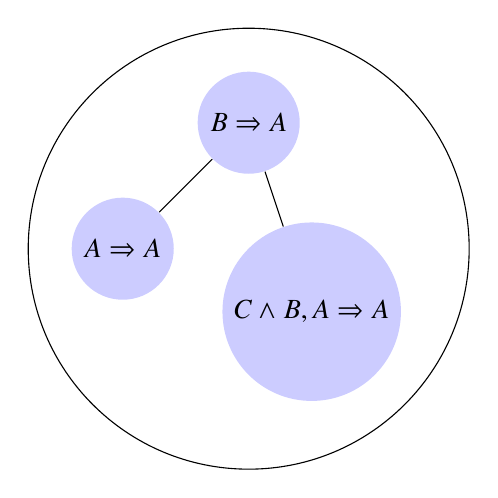
\begin{tikzpicture}
[scale=.8,auto=left,every node/.style={circle,fill=blue!20}]
\draw (3,3) circle (3.5);
\node (n1) at (1,3) {$A \Rightarrow A$};
\node (n2) at (3,5) {$B \Rightarrow A$};
\node (n3) at (4,2)  {$C \wedge B, A \Rightarrow A$};
\foreach \from/\to in {n1/n2,n2/n3}
\draw (\from) -- (\to);

\end{tikzpicture}


, if
 If $C$ $I(\Gamma \Rightarrow A)=1$ then
so does $I(\Pi, \Box \Gamma \Rightarrow \Box A, \Delta) = 1$ for example:
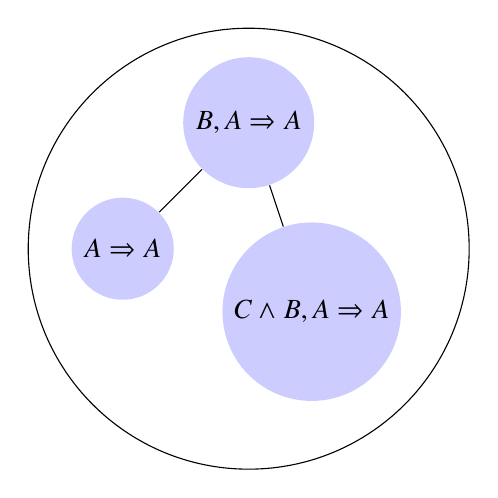
\begin{tikzpicture}
[scale=.8,auto=left,every node/.style={circle,fill=blue!20}]
\draw (3,3) circle (3.5);
\node (n1) at (1,3) {$A \Rightarrow A$};
\node (n2) at (3,5) {$B, A \Rightarrow A$};
\node (n3) at (4,2)  {$C \wedge B, A \Rightarrow A$};
\foreach \from/\to in {n1/n2,n2/n3}
\draw (\from) -- (\to);

\end{tikzpicture}

Therefore $R_k$ is sound.

% I just don't know how to explain this crap.

\section{}
\subsection{Prove $\Box p \Rightarrow \Box \Box p$}
Prove that the sequent $\Box p \Rightarrow \Box \Box p$, where $p$ is a
propositional variable, is not derivable in $GKC_k$.

A propositional variable is either true or false (boolean). To prove 
$\Box p \Rightarrow \Box \Box p$ is not derivable in $GKC_k$ we assume
it is derivable and try to construct a prove towards it from the axioms.

The Ax ($\Gamma, A \Rightarrow A \Delta$) Axiom cannot be used because it
doesn not contain propositional vraibles. So we're left with the 
$L\bot(\Gamma \bot \Rightarrow \Delta)$ and $R\top(\Gamma \top
\Rightarrow \Delta)$ axioms
\subsubsection{$L\bot$}
\begin{prooftree}
\end{prooftree}


\subsection{Prove $\Box A \to \Box \Box A$ }
Prove that $\Box A \to \Box \Box A$ holds in all transitive Kripke models.


\subsection{Explain why 2.1 and 2.2 imply incompletness}
Explain why 2a and 2b imply that K is not complete with respect to
transitive Kripke models.
\section{Prove, for any propositional}
Let G denote the calculus GKC extended by the rule
\begin{prooftree}
	\AxiomC{$\Box \Gamma, \Gamma \Rightarrow A$}
	\RightLabel{$R$}
	\UnaryInfC{$\Box \Gamma \Rightarrow \Box A$}
\end{prooftree}
Prove, for any variable $p$, that $\Box p \Rightarrow \Box \Box p$ is
not provable in G. Prove that not every sequent provable in $GKC_{K4}$
is provable in G. 
\subsection{Does the converse hold?}
%Yes or no, maybe a because
\section{Prove, using soundness}
Prove using sondness, that $GKC_K$ does not derive $(\Box A \Rightarrow A)$.

\section{Prove, that if $\vdash_{GKC_K}$}
Prove that if $\vdash_{GKC_K}(\Rightarrow \Box A)$, then 
$\vdash_{GKC_K}(\Rightarrow A)$

\end{document}
